\chapter{Background Information}
\label{ch:background-information}

In this chapter we will cover in brief the basic notion regarding the methodology we propose for the detection of words dificulty. The methodology itself is described in chapter \ref{ch:methodology}.

\section{Classification problem}
Classification is a supervised machine learning problem. Given a set
of $n$ attributes (features), a set of $k$ classes and described by a set of $m$ labeled training instances $$\{(x_i,y_i); i=1,...,m\},$$ where $x_i$
is a feature vector and $y_i$  is a label, the task is to find such a
model, which predicts the class of any instance from the values of its attributes.

A lot of real-world problems can be considered as a classification problem, for instance \citep{Ng-2012cs229}:
\begin{itemize}
    \item understanding whether a tumor is malignant or benign by its size,
    \item distinguishing spam and non-spam emails by the words they contain,
    \item identifying fraudulent transactions among normal ones using their metadata.
\end{itemize}
To handle those tasks a lot of classification algorithms currently exist, among which the most commonly used groups are linear classifiers, support vector machines, nearest neighbors classifiers, decision trees, artificial neural networks.

We will concentrate on the last two further in this chapter.

\subsection{Classifier performance evaluation}
\label{sec:clf-eval}

When training any machine learning model, the full set of available data is commonly split into several parts:
\begin{enumerate}
    \item Training set - the sample of data used for training (fitting) a model. This is the only set with target variable (labels in case of classification) "visible" for a model. In the case of all the rest of datasets, the target variable is only used for performance evaluation of the fitted model. 
    \item Validation or development set - the sample of data used for unbiased evaluation of model fit on training set while tuning model's hyperparameters. In other words, this set is needed to choose a model which will be finally used in production.
    \item Test set - the sample of data used for unbiased evaluation of the final model, which was fitted on training dataset \citep{Kuhn-2013}.
\end{enumerate}

To evaluate a classification model predicted labels results are compared with class labels provided in development or test set. This allows checking the generalization ability of the model.

For simplicity of the explanation how a classifier is evaluated, we will consider evaluation of a binary classifier, which has only two target classes for prediction: positive and negative. 
Binary classifiers are mostly evaluated using confusion matrix (fig. \ref{fig:confusion-matrix}).

\begin{figure}[h]
    \centering
    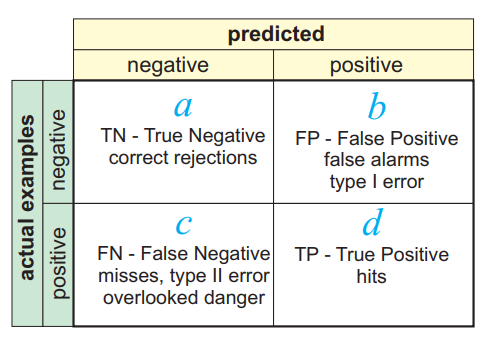
\includegraphics[width=8cm]{Images/Confusion-matrix.png}
    \caption{Confusion matrix. Source: \citep{kohavi:glossary}.}
    \label{fig:confusion-matrix}
\end{figure}

Performance measures calculated from the confusion matrix entries are
the following \citep{Sebastiani2002}:
\begin{itemize}
    \item Accuracy $= (a + d)/(a + b + c + d) =
    (TN + TP)/total$ ;
    \item True positive rate, recall, sensitivity$ =
    d/(c + d) = TP/actual\: positive$ ;
    \item Specificity, true negative rate $= a/(a + b) =
    TN/actual\: negative$ ; 
    \item Precision, predicted positive value $=
    d/(b + d) = TP/predicted\: positive$ ;
    \item False positive rate, false alarm $= b/(a + b)
    = FP/actual\: negative = 1 - specificity$ ;
    \item False negative rate $= c/(c + d) = FN/actual\: positive$ .
\end{itemize}

One of the measures above is not enough to evaluate a binary classifier properly when data is class imbalanced. For instance, on fig. \ref{fig:classifiers-evaluation} the accuracy is high and equal for both situations, but precision and recall differ significantly. 

\begin{figure}[h]
    \centering
    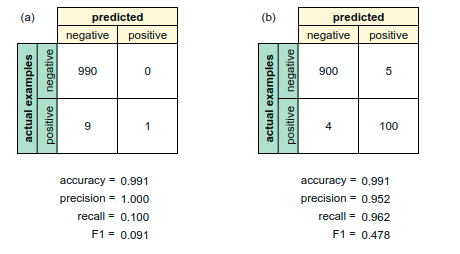
\includegraphics[height=8cm]{Images/Classifiers-evaluation.png}
    \caption{Examples of classifiers evaluation.}
    \label{fig:classifiers-evaluation}
\end{figure}

Moreover, it is always a question what to prioritize, precision or recall, and how to find balance among these two measures. For this reason, $F_1$ score, a harmonic mean of precision and recall \citep{Chinchor-1992}, is frequently used to evaluate a binary classifier:

\begin{equation}
    F_{1}=2\cdot {\frac {\mathrm {precision} \cdot \mathrm {recall} }{\mathrm {precision} +\mathrm {recall} }}
\end{equation} 

In our experiments described in chapter \ref{ch:experiments} we work with multiclass classification problem on unbalanced datasets (Table \ref{tab:annot-results}). The quality of the applied classification algorithms is evaluated using four standard measures: accuracy $A$, precision $P$, recall $R$ and F1-measure $F$. To effectively measure the ability of a model to distinguish between three target classes of words in an unbalanced dataset we use \textit{macroaveraging} of three one-vs-rest binary classifiers. Macroaveraging is a method to measure multiclass classifier in case of unbalanced dataset \citep{Sebastiani2002}. Precision and recall are first evaluated `locally' for each class and then `globally' by averaging over the results of the different categories:

\begin{equation}
    P^M = \dfrac{\sum_{i=1}^{|C|} P_i}{|C|},\: R^M = \dfrac{\sum_{i=1}^{|C|} R_i}{|C|},
\end{equation}

where:
\begin{conditions}
 M      & for macroaveraging, \\
 C &  $\{c_1, ..., c_{|C|}\}$ - set of classes,\\ 
 |.| &  capacity (number of samples),  \\   
 |C| & total number of samples in the dataset.
\end{conditions}

\subsection{Cross-validation}
\label{sec:cross-val}

\textit{Cross-validation} (also called \textit{out-of-sample testing} or \textit{rotation estimation}) is a model validation technique for assessing how the results of a statistical analysis will generalize to an independent data set \citep{Kohavi-1995}. To perform a cross-validation the full dataset $D$ is randomly split into $k$ mutually exclusive subsets (the \textbf{folds}) $D_1, D_2, ..., D_3$ of approximately equal size. Then the model is trained and tested $k$ times. Each time $t \in \{1,2,...,k\}$ it is trained on all fords except for $t^{th}$ one: $D\D_t$, - and tested on $D_t$. The chosen performance measure $\pi$ is calculated at each time $t$ on test set and then averaged resulting to cross-validation performance estimate: $\pi_{CV} = 1/n \sum_{t=1}^{k}\pi_i$.

Mostly cross-validation is performed within the instances of dataset (rows in case of table data). Whereas in this work we propose to cross-validate also within different target columns (annotations) and within instances and target columns simultaneously (chapter \ref{ch:methodology}).

\section{Decision trees}
Decision trees can be used for both regression and classification tasks. Learning a decision tree is the construction of a tree-like model out of class-labeled training tuples. An example of a decision tree is shown on fig. \ref{fig:decision-tree}. Such model is, in fact, a sequence of conditional control statements based on values of feature vectors characterizing input observations. 

\begin{figure}[h]
    \centering
    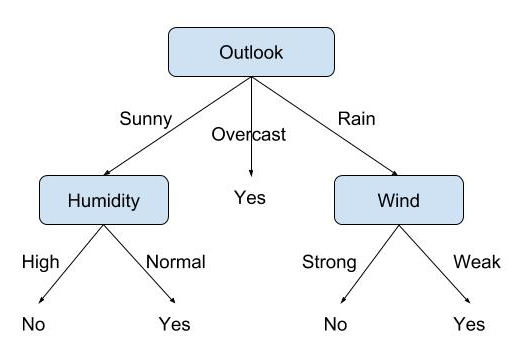
\includegraphics[width=8cm]{Images/Decision-tree.png}
    \caption{A decision tree for decision making about playing tennis on the day.}
    \label{fig:decision-tree}
\end{figure}
% \includegraphics[height=5cm]{Decision tree} 

A decision tree is mostly learned using the recursive binary splitting technique. In this process on each step, an algorithm is aimed to find the best feature and splitting condition to finally come up with the shortest path to the final decision.
Learning an optimal binary decision tree in such a way is an NP-complete problem \citep{Hyafil-1976}. For this reason on practice greedy heuristic algorithms are used, where locally optimal decisions are made at each node. In this work we use an implementation of popular ID3 (Iterative Dichotomiser 3) algorithm \citep{Quinlan-1986} in all our experiments \ref{ch:experiments}. Using decision trees in applications of evidence-based medicine is common as this model is conceptually simple, provides high accuracy and mimics the way a doctor thinks \citep{Sackett-1996, Podgorelec-2002}. Moreover, decision trees give clear explanation of the class choice, which is valuable for medicine where it is important to have the traceability of the results. For NLP tasks deision trees similarly provide valuable information on the relevant features and/or feature values.

To sum up, the advantages of decision trees are:
\begin{itemize}
    \item simplicity of concept and interpretability,
    \item possibility to apply to both categorical and numeric data without a need of regularization,
    \item easiness to combine with other decision techniques.
\end{itemize}

Disadvantages of decision threes are:
\begin{itemize}
    \item instability - a small change in data can lead to a dramatic change in the model,
    \item propensity of overfitting if no constraints are put. To avoid this effect in our experiments, we restricted the depth of trees as specified in tables of chapter \ref{ch:experiments}.
\end{itemize}


\section{Artificial neural networks}
An Artificial Neural Network (ANN) is a mathematical model which consists of interconnected layers of neurons (groups of nodes) as shown on fig. \ref{fig:neural-net}. Layers can be of different types, and it is common to stack several distinct layers together in a specific manner to get a neural network with good performance. The model on fig. \ref{fig:neural-net} contains two \textit{fully-connected} hidden layers where neurons are fully pairwise connected between two adjacent layers \citep{FeiFei-2016}. Artificial neural networks with contain multiple hidden layers are called Deep Neural Networks (DNN). 

\begin{figure}[h]
    \centering
    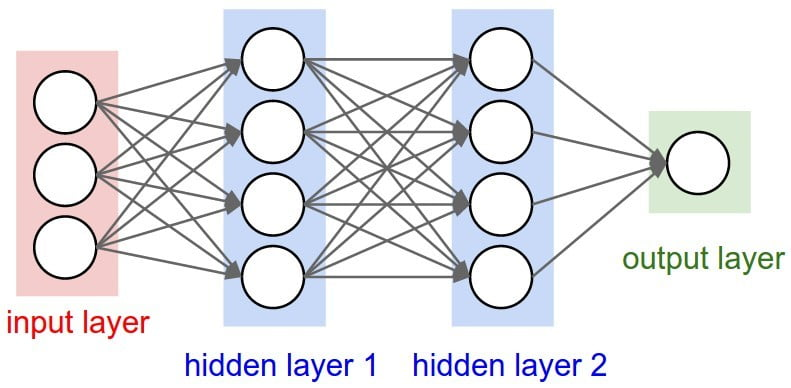
\includegraphics[width=8cm]{Images/Neural-network.jpg}
    \caption{A 3-layer neural network with three inputs, two hidden layers of 4 neurons each and one output layer. Source: \citep{FeiFei-2016}}
    \label{fig:neural-net}
\end{figure} 

A neural network can be used for both supervised and unsupervised tasks. In the case of supervised training (such as classification), the network processes inputs and provides outputs (predictions). Predictions are then compared with the correct values of target variable values. Errors are then propagated back through the system. This process results in adjusted weights of a neural network. The aim is after many iterations of the described procedure to receive well-tweaked weights of the neural network which provide satisfactory performance of the model. 

As ANNs contain a lot of connections (which are expressed as weights in mathematical model), much data needs to pass through the model to train it well. As the data passed to model is stored in random-access memory (RAM) of the working machine during forward and backward passes, we mostly cannot pass all the available data at once to our model. That is why data is split by small portions called \textit{batches}. A complete pass of a given dataset through the model is called \textit{epoch}. It is one iteration of learning. The different number of epochs is needed to learn different DNN architectures, from 5 to hundreds. In this work, we trained neural networks for at most 16 epochs, which was enough for our task.

\subsection{Recurrent neural networks}
\label{sec:rnn}
A Recurrent Neural Network (RNN) is a type of ANN for handling sequential data by processing them element-wise and storing in the internal memory (hidden state). A part of an RNN is presented on fig. \ref{fig:rnn}.

\begin{figure}[h]
    \centering
    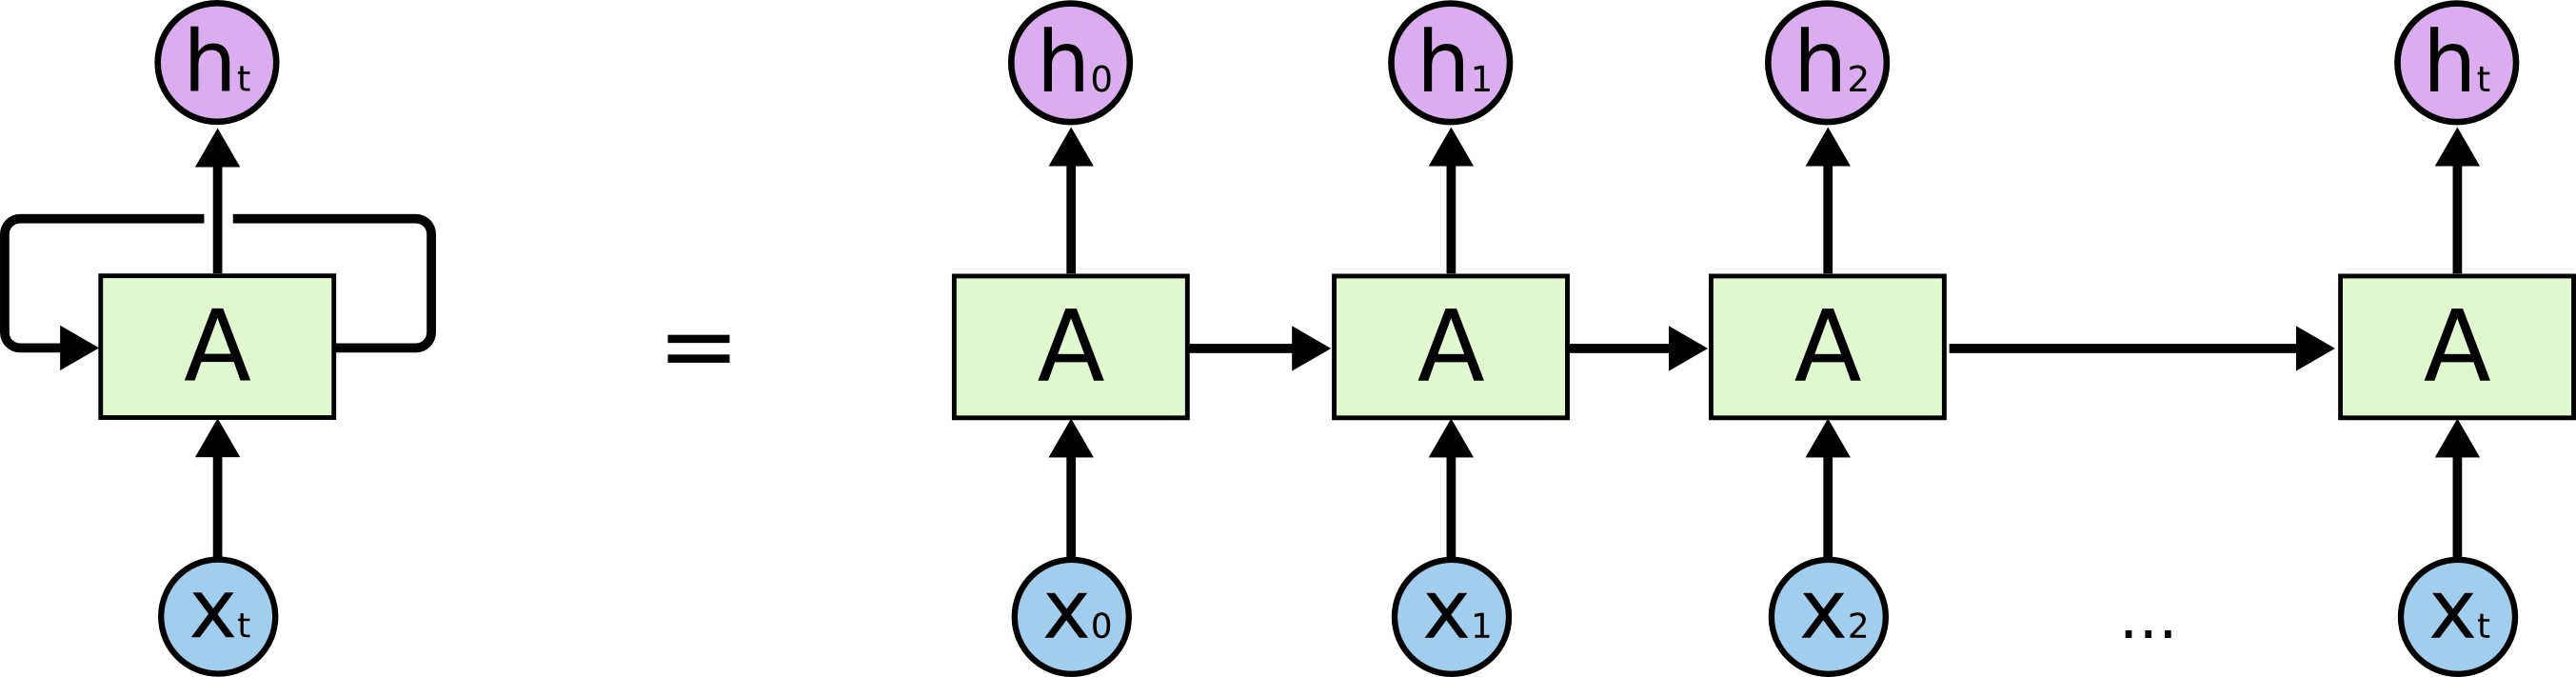
\includegraphics[width=10cm]{Images/RNN-unrolled.png}
    \caption{A rolled (on the left) and unrolled (on the right) part of vanilla (or conventional) RNN. At each time step $t$ the model takes the $t^{th}$ member of sequence $x_t$ and outputs a hidden state value $h_t$. Source: \citep{Olah-2015}}
    \label{fig:rnn}
\end{figure} 

Formally, forward propagation of an RNN begins with initialization of the initial hidden state $h^{(0)}$ and then for each time step from $t=1$ to $t=\tau$ the next update equations are applied \citep{Goodfellow-2016}:

\begin{equation}\label{eq:rnn}
\begin{gathered} 
    a^{(t)} = b+Wh^{(t-1)}+Ux^{t}, \\
    h^{(t)} = tanh(a^{(t)}), \\
    o^{(t)} = c+Vh^{(t)}, \\
    y^{(t)} = softmax(o^{(t)}),
\end{gathered}
\end{equation}
%%
where $x^{t}$ is an input vector, $y^{t}$ is an output vector and the parameters are weight matrices $U, V, W$ - for input-to-hidden, hidden-to-output and hidden-to-hidden connections respectively, and bias vectors $b$ and $c$.

Due to the specifics of RNNs, these models are widely used not only for solving classical NLP ones like machine translation \citep{Chen-2018} and part-of-speech tagging \citep{Plank-2016}, but also for handling sequence-based tasks from other domains like program code generation \citep{Stehnii-2017} and filling missing values in multivariate time series \citep{Che-2016}.

\subsubsection{Long short-term memory units}
\label{sec:lstm}
As it follows from fig. \ref{fig:rnn} the vanilla RNN processes information sequentially through the time in both directions, forward and backward. This means that the signal can be easily corrupted when multiplied on small numbers (near 0) several times. This is known as \textit{vanishing gradients} problem, when happends during backpropagation. This prevents a vanilla RNN from memorizing long-term dependencies.

Long short-term memory (LSTM) units are designed with idea to get rid of this problem. In LSTM the repeating model has different from vanilla RNN structure (fig. \ref{fig:lstm}). Instead of having a single neural network layer, there are four, interacting in a very special way. The key \textit{distinctive feature} of LSTM is the top horizontal line which runs down the entire chain with minor linear interactions. So the information flows with this part with almost no changes \citep{Olah-2015}.

\begin{figure}[h]
    \centering
    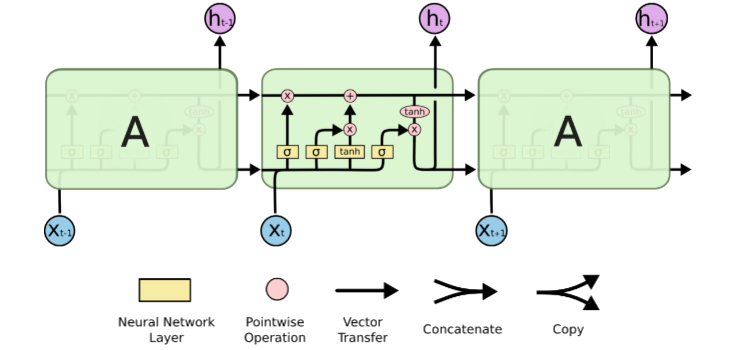
\includegraphics[width=10cm]{Images/lstm.png}
    \caption{The repeating module in an LSTM contains four interacting layers. Below are explanations of symbols used on the diagram. Source: \citep{Olah-2015}}
    \label{fig:lstm}
\end{figure} 

The vanilla LSTM and its modifications are frequently used for building sequence-processing systems and show advantage in performance compared to other RNN units \citep{Hochreiter-1997}.
In this work, after experimenting with different RNN architectures, an LSTM-based one showed the best results for our task \ref{appx:rnn}. 

\section{Vector words representations}

\textit{Word embedding} is a collective name for a set of language modeling and feature learning techniques in NLP where words or phrases from vocabulary are mapped to real-valued vectors in a predefined low-dimensional space. This concept is widely used nowadays in applications of NLP as working with word vectors of vocabulary size (thousands or millions of dimensions) is computationally hard. Whereas each high dimensional vector is sparse containing only a few "valuable" non-zero values, which led to the idea that words can be represented much more densely \citep{Harris-1954}. Mathematically this process involves a mathematical embedding from space with one dimension per word to a continuous vector space with a much lower dimension (mostly from 100 to 300 dimensions) \citep{Brownlee-2017}.

\begin{figure}[h]
    \centering
    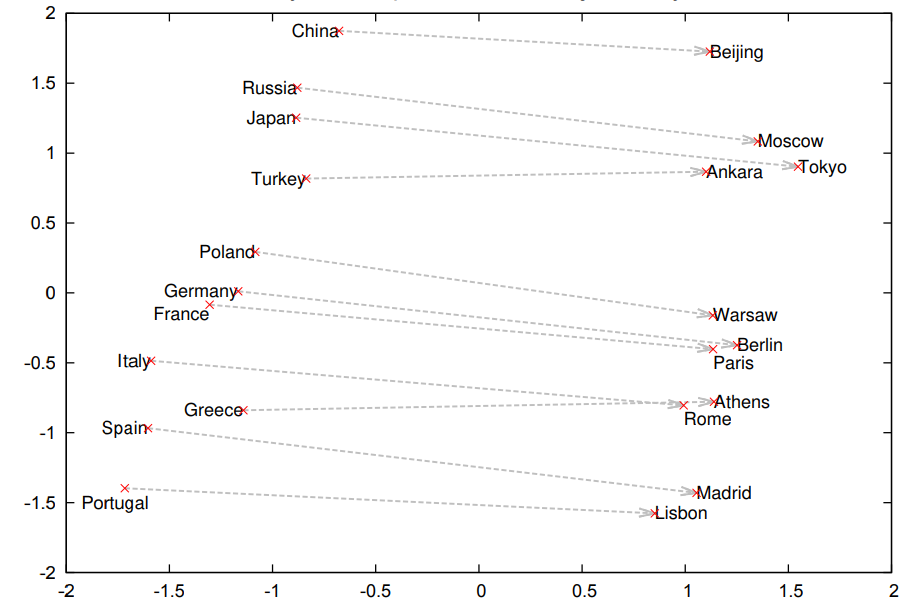
\includegraphics[height=8cm]{Images/word2vec-property.png}
    \caption{Country and Capital Vectors Projected by PCA (Principal Component Analysis). The figure illustrates the ability of the word2vec model to organize concepts and learn the relationships between them implicitly. No supervised information about country-capital correspondence was provided to model during learning. Source: \citep{Mikolov-NIPS2013}}
    \label{fig:word2vec-property}
\end{figure} 


\subsection{Word2vec} 
\label{sec:word2vec}
Word2vec is a well-known deep-learning-based approach for receiving word embeddings which has seen tremendous success being applied in numerous NLP tasks due to its computationally-efficiency and high quality of result \cite{Mikolov-NIPS2013}. Word2vec representations can be trained using either skip-gram model \citep{Mikolov-NIPS2013} shown on fig. \ref{fig:word2vec-skip-gram}  or Continuous Bag-of-Words model (CBOW) \citep{Mikolov-ICLR2013} shown on fig. \ref{fig:word2vec-cbow}.

\begin{figure}[h]
    \centering
    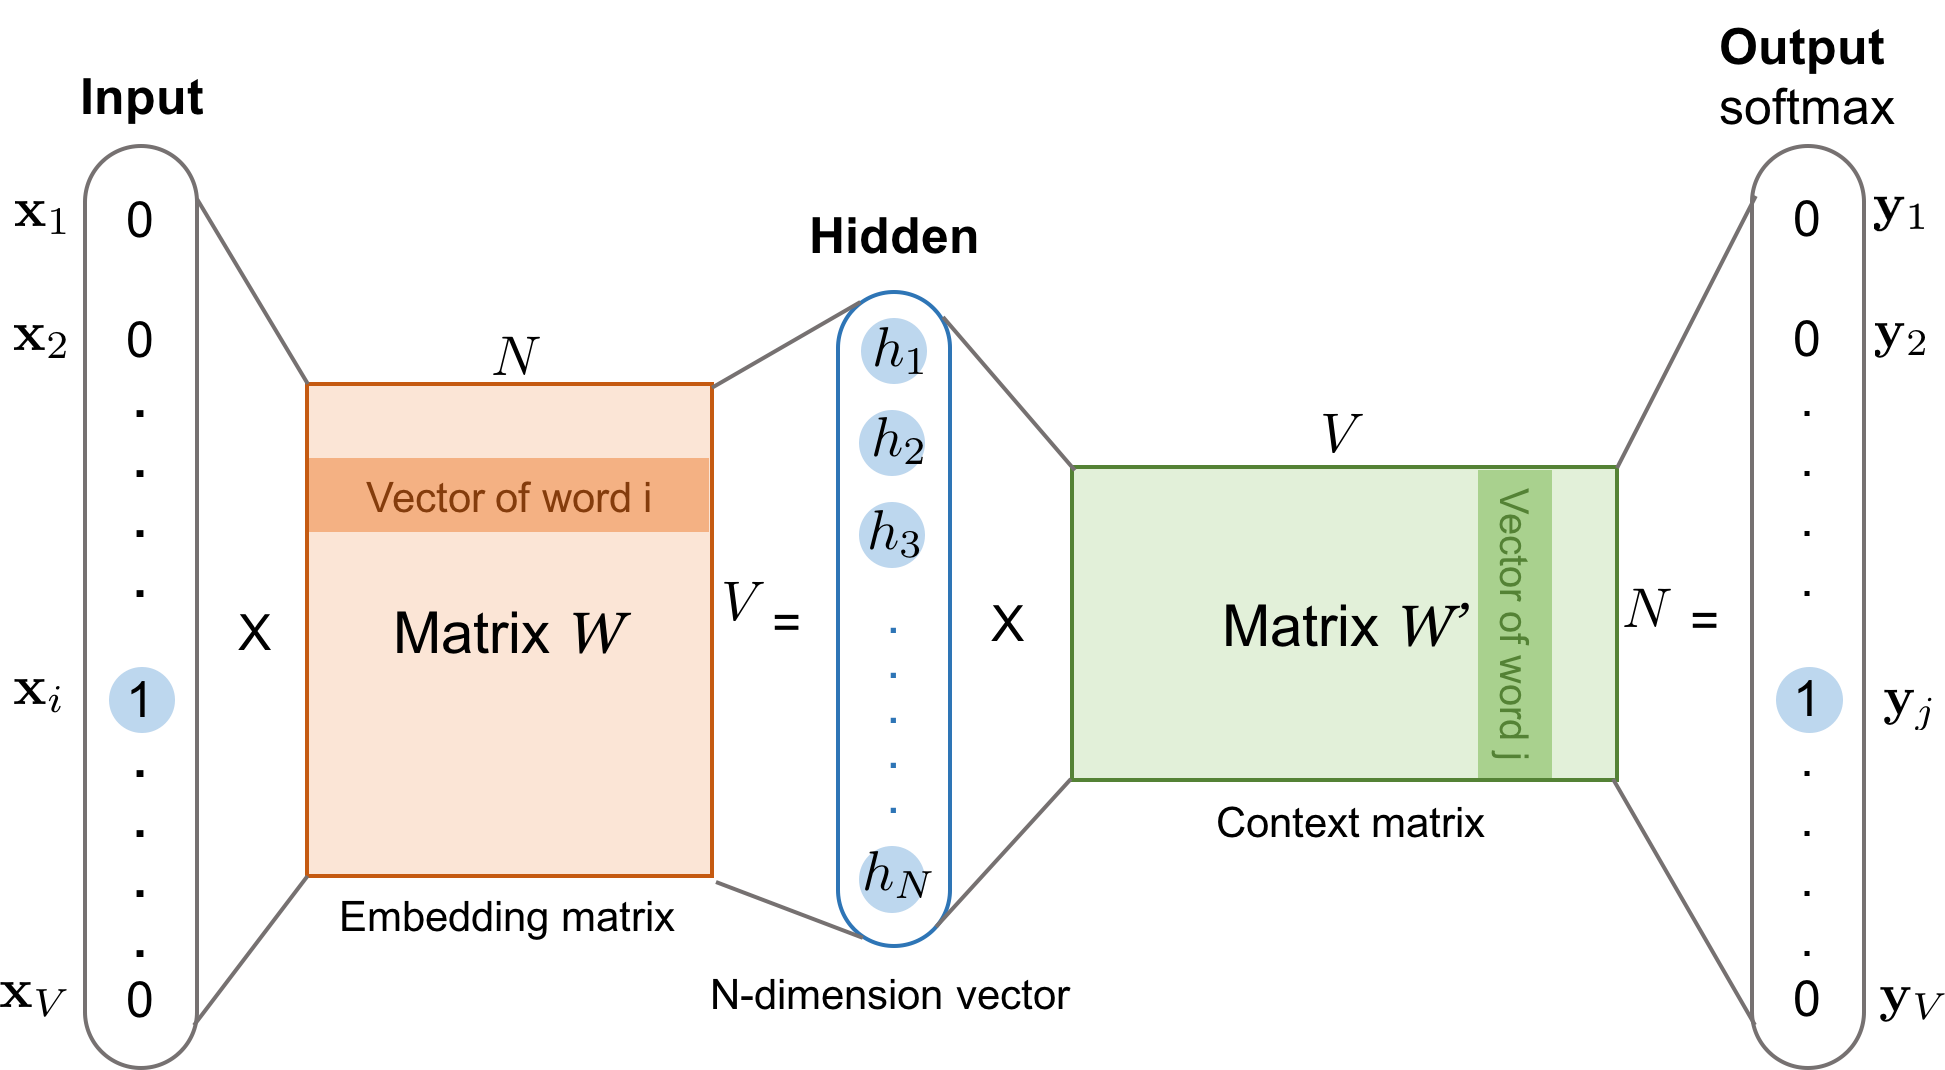
\includegraphics[height=4.5cm]{Images/word2vec-skip-gram.png}
    \caption{The skip-gram model. Both the input vector $x$ and the output $y$ are one-hot encoded word representations. The hidden layer is the word embedding of size $N$. Source: \citep{Weng-2017}}
    \label{fig:word2vec-skip-gram}
\end{figure} 

\begin{figure}[h]
    \centering
    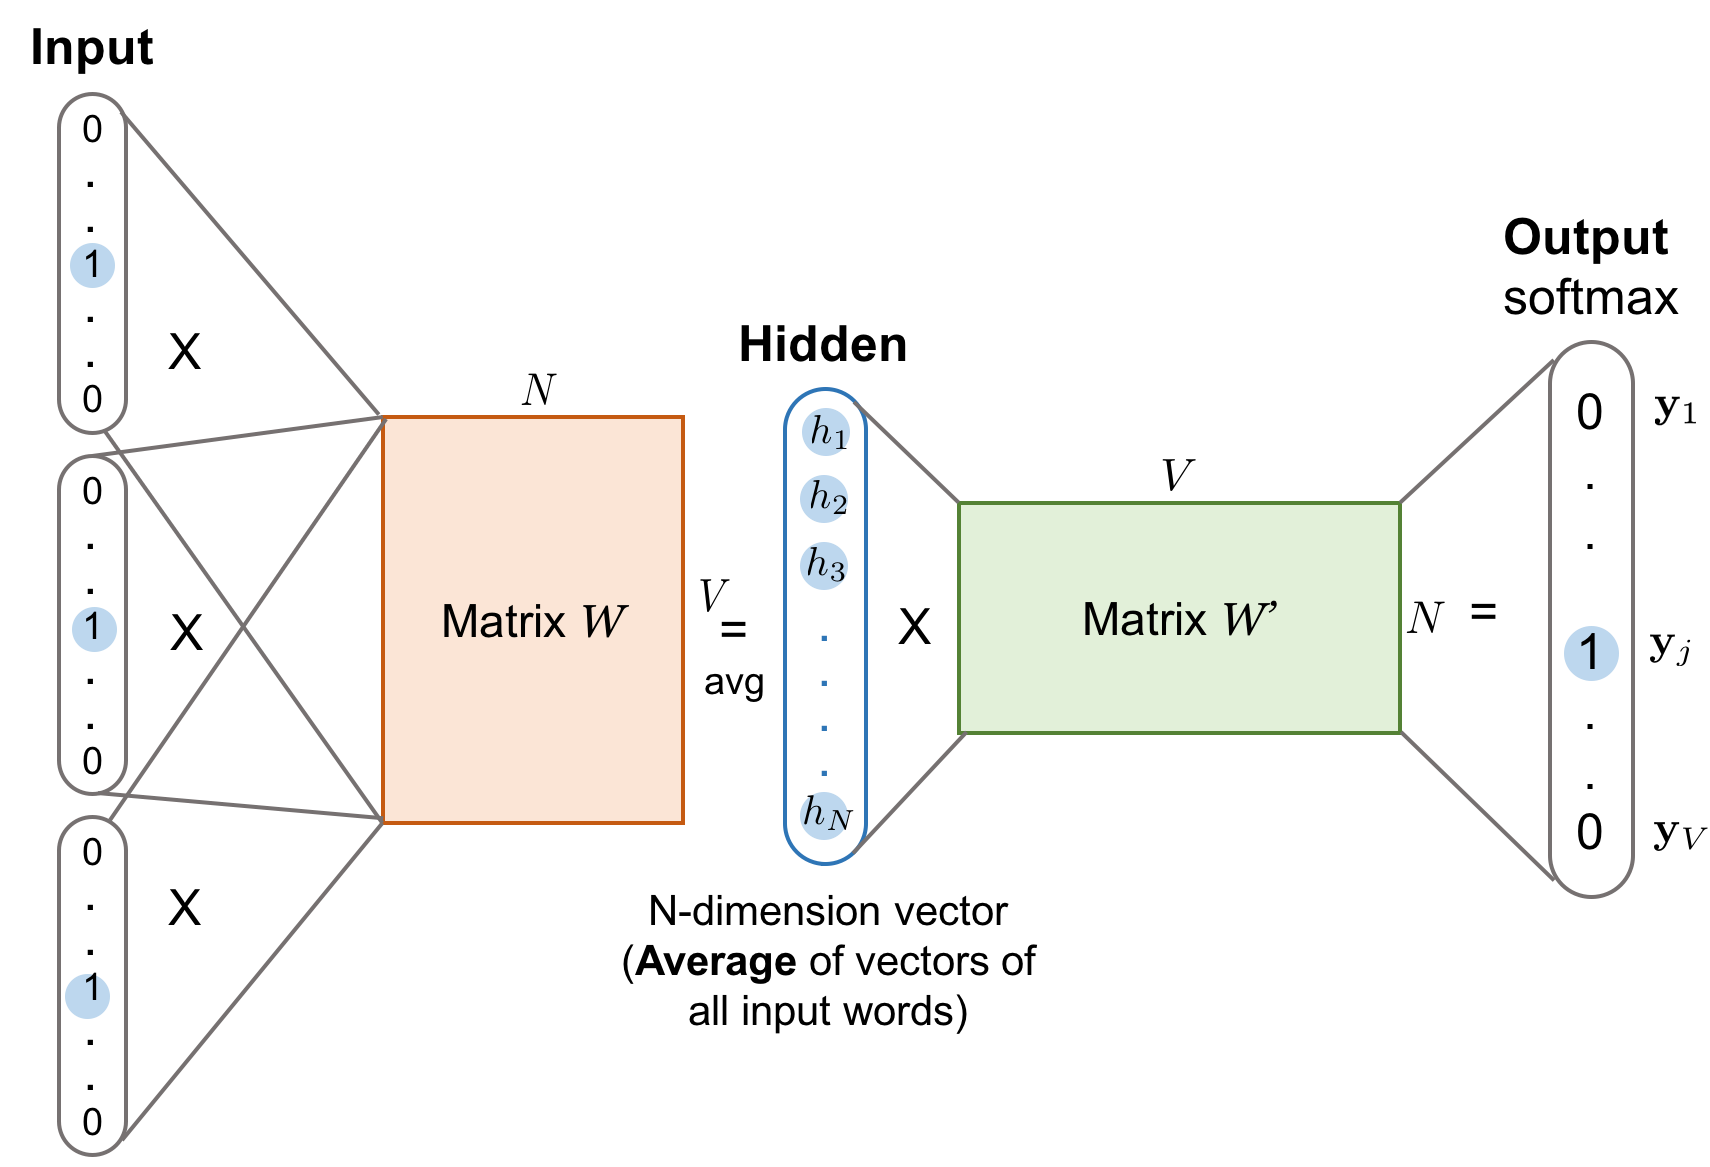
\includegraphics[height=5cm]{Images/word2vec-cbow.png}
    \caption{The CBOW model. Word vectors of multiple context words are averaged to get a fixed-length vector as in the hidden layer. Source: \citep{Weng-2017}}
    \label{fig:word2vec-cbow}
\end{figure} 

A nice property of word2vec words representation is that due to the way word embeddings are learned, final vectors capture context information of words, which results in the existence of semantic word relationships, an example of which is shown on fig. \ref{fig:word2vec-property}. 

For this reason, such vectors are frequently used as features for many canonical NLP prediction tasks, such as part-of-speech tagging, named entity recognition \citep{Collobert:DBLP}, or classification. In our work for the same purpose, we utilized fastText word embeddings - an advanced modification of word2vec model.

\subsection{FastText word representations}
\label{sec:fasttext}

In NLP applications it is common to use pre-trained word representations estimated from a large corpus of non-domain-specific texts: news collections, Wikipedia, Web Crawl. In vanilla word2vec setting word embeddings map each word to a distinct vector ignoring morphology. Moreover, words with low frequency in training corpora might be excluded from the final set of word-vector correspondences. This leads to a need of handling the problem of out-of-vocabulary (OOV) words when applying pre-trained word representations on a new corpus. When the domain of new texts contains much specific terminology, as in the case of our dataset of medical terms described in Chapter \ref{ch:dataset-description}, OOV problem becomes tough to resolve.

FastText is a skip-gram model trained on \textit{n-grams} level
introduced in \cite{Bojanowski-ACL2017}. In this approach, each word
is represented as a sum of character n-gram representations of this word's
components. This makes it easy to represent any OOV word. Pre-trained word vectors for 157 languages using fastText were received and made public \footnote{\url{https://fasttext.cc/docs/en/crawl-vectors.html}} by Facebook AI Research in 2017 \citep{Mikolov-2017}. The results of applying those vectors for the French language on our dataset are described in \ref{sec:cv-experiments}.

FastText embedding vectors are the sum of character n-gram representations, so that they could be generated even for unknown words. 


\bigskip
In this chapter we provided the background information which briefly describes all the components of our proposed methods. In the next chapter we will describe the dataset used in experiments.